\documentclass{cvf}
\usepackage{amssymb}

\begin{document}

\chapter{Curriculum Vitae}

\begin{tabular}{c|c}
\begin{minipage}{10cm}
\name{Jorge Alda Gallo}
\vspace{0.8cm}
\presentation{Ph.D. in Theoretical Physics}
\noindent
\email{jalda@unizar.es}
\phone{+34 676 70 35 11}
\address{C/Rioja 18 2B, 50017 Zaragoza, Spain.}
\webpage{https://jorge-alda.github.io}
\github{Jorge-Alda}
\orcid{0000-0002-6728-1105} 
\end{minipage} & \hspace{1cm} 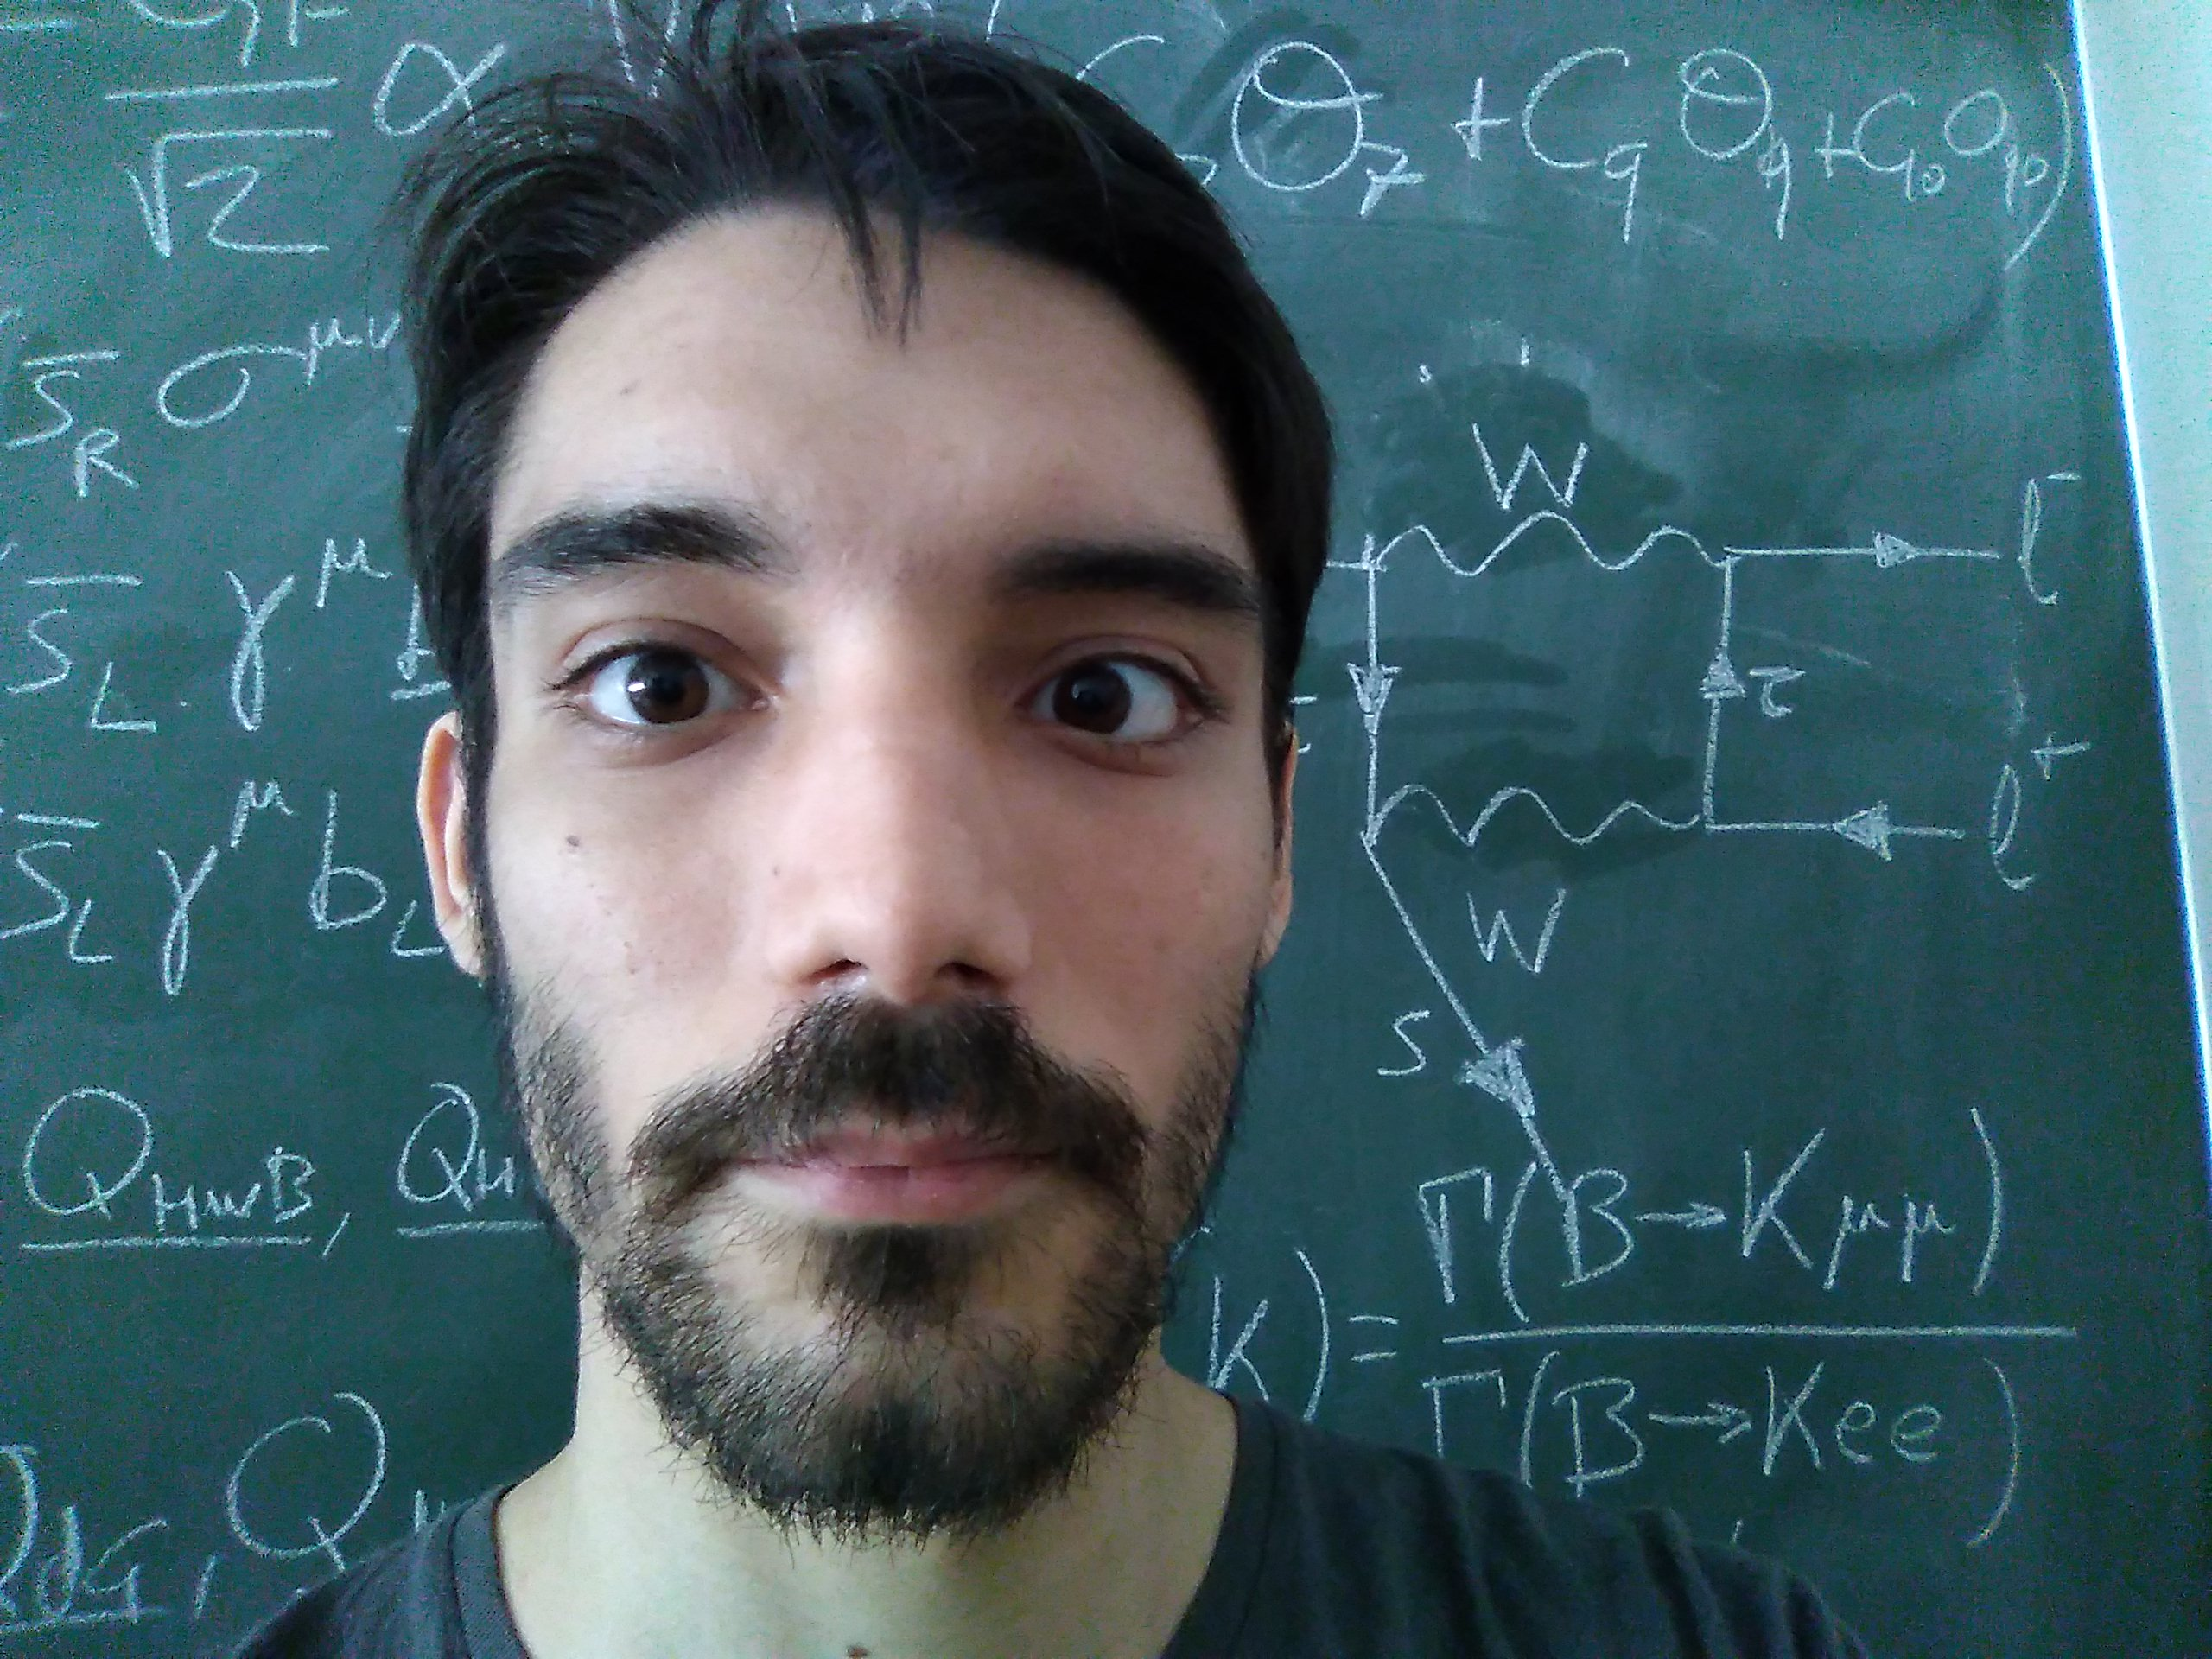
\includegraphics[width=4cm]{photo.jpg}
\end{tabular}

\interests{Research interests}
\begin{itemize}
\item New physics beyond the Standard Model.
\item Flavour Physics.
\item $B$-meson anomalies.
\item Effective Field Theories.
\item Axions and Axion-like particles.
\end{itemize}

\education{Education}
\datedsubsection{B.Sc. in Physics, Universidad de Zaragoza}{2011-2015}
Average grade: 9.20/10. 13 Honours.\\
B.Ss. Project: \textit{``Cálculo numérico en teoría cuántica de campos de la materia condensada''}. Under the supervision of David Zueco Láinez. Qualification: 9.5/10.

\datedsubsection{M.Sc. in Theoretical Physics, Universidad Complutense de Madrid}{2015-2016}
Average grade: 9.34/10.\\
M.Sc. Project: \textit{New Applications of the Coleman-Weinberg Model}. Under the supervision of J. A. Ruiz Cembranos. Qualification: 9.0/10.

\datedsubsection{Ph.D. School}{2018}
Taller de Altas Energías. Benasque (Huesca, Spain).

\datedsubsection{Ph.D. in Physics, Universidad de Zaragoza}{2016-2022}
Under the supervision of Siannah Peñaranda Rivas.\\
Dissertation title: \textit{A Glance into Flavour Physics with Effective Field Theories and Machine Learning}.

\grants{Grants}
\datedsubsection{Grant JAE-Intro CSIC}{2014}
Project \textit{``Caos semiclásico en sistemas de bosones con interacción''}, supervised by David Zueco Láinez.\\
CSIC-ICMA (Spanish National Research Council and Instituto de Ciencia de Materiales de Aragón).

\datedsubsection{PreDoc Grant, Diputación General de Aragón}{2017-2022}

\datedsubsection{Programa Ibercaja-CAI de Estancias de Investigación}{2021}
Grant No. CB 5/21.

\memberships{Memberships}
\datedsubsection{CAPA}{2019-present}
Centro de Astropartículas y Física de Altas Energías. Zaragoza, Spain.\\
\url{capa.unizar.es}

\invited{Invited Positions}
\datedsubsection{Università degli Studi di Padova/INFN}{Summer 2021}

\works{Scientific Production}

\hspace{\parindent}
\textbf{J. Alda, J. Guasch and S. Peñaranda: \textit{Some results on Lepton Flavour Universality Violation}}\\
Eur.Phys. J. C, 79 7 (2019) 588\\
doi:10.1140/epjc/s10052-019-7092-x\\
arXiv:1805.03636 [hep-ph]

~

\textbf{J. Alda, J. Guasch and S. Peñaranda: \textit{Anomalies in $B$ decays: A phenomenological approach}}\\
arXiv:2012.14799 [hep-ph]\\
Accepted for publication in The European Physical Journal Plus.

~

\textbf{J. Alda, J. Guasch and S. Peñaranda: \textit{Anomalies in $B$ decays: Present status and future collider prospects}}\\
arXiv:2105.05095 [hep-ph]\\
SLAC eConf C21-03-15.1

~

\textbf{J. Alda, J. Guasch and S. Peñaranda: \textit{Using Machine Learning techniques in phenomenological studies in flavour physics}}\\
arXiv:2109.07405 [he-ph]

~

\textbf{J. Alda, J. Guasch and S. Peñaranda: \textit{Exploring B-physics anomalies at colliders}}\\
arXiv:2110.12240 [hep-ph]\\
PoS(EPS-HEP2021)494

~

\textbf{J. Alda, A. W. M Guerrera, S. Peñaranda and S. Rigolin: \textit{Leptonic Meson Decays into Invisible ALP}}\\
arXiv:2111.02536 [hep-ph]

\conferences{Talks and conferences}

\hspace{\parindent}\textbf{2nd Red LHC Workshop. Madrid, Spain. 9-11 May 2018}\\
Talk ``Some Results on Lepton Flavour Violation''.

~

\textbf{Taller de Altas Energías. Benasque (Huesca, Spain) 2-15 September 2018}\\
Talk ``Some Results on Lepton Flavour Violation''.

~

\textbf{X CPAN Days. Salamanca, Spain. 29-31 October 2018}\\
Talk ``Complex Wilson coefficients in the analysis of $B$-anomalies''.

~

\textbf{I Jornadas de Jóvenes Investigadores CAPA. Zaragoza, Spain. 7 May 2019}\\
Talk ``Effective Theories for $B$-meson anomalies''.

~

\textbf{I Jornadas del Programa de Doctorado de Física. Zaragoza, Spain. 20 June 2019}\\
Talk ``Effective Theories for $B$-meson anomalies''.

~

\textbf{XXXVII Bienal de Física de la Real Sociedad Española de Física. Zaragoza, Spain. 15-19 de July 2019}\\
Talk ``Some Results on Lepton Flavour Universality Violation''.

~

\textbf{International Workshop on Future Linear Colliders - LCWS2021. Online. 15-18 March 2021}\\
Talk ``Anomalies in $B$ mesons decays: Present status and future collider prospects''.

~

\textbf{European Physical Society Conference on High Energy Physics 2021 (EPS-HEP2021). Online. 26-30 July 2021}\\
Poster ``Exploring B-physics anomalies at colliders ''.

~

\textbf{Seminar, Department of Theoretical Physics. University of Zaragoza, Spain. 18 November 2021}\\
Talk ``Leptonic Mesons Decays into invisible ALP''.

~

\textbf{II Jornadas del Programa de Doctorado de Física. University of Zaragoza, Spain. 3 December 2021}\\
Talk ``Leptonic Mesons Decays into invisible ALP''.

~

\textbf{Seminar, Department of Theoretical Physics. University of Zaragoza, Spain. 20 January 2022}\\
Talk ``Using Machine Learning techniques in phenomenological studies in flavour physics''.

~

\textbf{Seminar, Institute of Theoretical Physics (IFT). Autonomous University of Madrid, Spain. 27 January 2022}\\
Talk ``Using Machine Learning techniques in phenomenological studies in flavour physics''.

\repositories{Contributions to public repositories}

\subsection{flavio}
1 pull request merged: \url{https://github.com/flav-io/flavio/pull/160}

\subsection{smelli}
1 pull request: \url{https://github.com/smelli/smelli/pull/45}

\teaching{Teaching}

\subsection{September 2019}
\hspace{\parindent}\textbf{Ph.D. School ``Taller de Altas Energías de Benasque'' (Huesca, Spain).}\\
Associate teacher.

\subsection{2019-2020}
\hspace{\parindent}\textbf{Differential Equations}\\
Problem-solving sessions, 38 teaching hours.\\
Second year course, Bachelor Degree in Physics, Universidad de Zaragoza.

~

\textbf{General Physics}\\
Laboratory sessions, 10 teaching hours.\\
First year course, Bachelor Degree in Mathematics, Universidad de Zaragoza.

\subsection{2020-2021}
\hspace{\parindent}\textbf{Differential Equations}\\
Problem-solving sessions, 38 teaching hours.\\
Second year course, Bachelor Degree in Physics, Universidad de Zaragoza.

~

\textbf{General Physics}\\
Laboratory sessions, 10 teaching hours.\\
First year course, Bachelor Degree in Mathematics, Universidad de Zaragoza.

\subsection{2021-2022}
\hspace{\parindent}\textbf{Differential Equations}\\
Problem-solving sessions, 38 teaching hours.\\
Second year course, Bachelor Degree in Physics, Universidad de Zaragoza.

~

\textbf{Co-direction of B.Sc. Project}\\
10 teaching hours.
Fourth year course, Bachelor Degree in Physics, Universidad de Zaragoza.

~

\textbf{General Physics}\\
Laboratory sessions, 10 teaching hours.\\
First year course, Bachelor Degree in Mathematics, Universidad de Zaragoza.

\languages{Languages}
\begin{tabular}{ll}
Spanish & \level{5} \\
English & \level{5} \\
Italian & \level{3} \\
German & \level{3} \\
French & \level{2}
\end{tabular}

\coding{Coding languages}
\begin{tabular}{ll}
\TeX/\LaTeX & \level{5}\\
Python & \level{5}\\
C/C++ & \level{3}\\
Mathematica & \level{3}
\end{tabular}

\awards{Awards}
\datedsubsection{XXII Spanish Physics Olympiad}{2011}
Silver Medal (Rank 15).\\
Second position in the regional Aragonese phase.

\datedsubsection{20th International Mathematics Competition}{2013}
Bronze Medal (rank 177).

\newpage

\section{About this CV}
\begin{tabular}{L{10.5cm}C{5.5cm}}
\begin{minipage}[b]{10cm}
This CV was last updated in \today.\\
You can find the latest version at \\ \url{https://github.com/Jorge-Alda/Jorge-Alda/releases/latest/download/CV.pdf}
\end{minipage} & \includegraphics[width=3cm]{qrcode.png}
\end{tabular}


\end{document}